\chapter{Project Management}
\label{chap:final-project-management}

\todo{The milestones were meant to be adjustable based on how the project go}

To avoid getting overwhelmed with the latest \gls{nlp} papers in the field of \gls{qa} systems, and \glspl{gs}, the author defined workflow components to gather valuable information:

\begin{itemize}
    \setlength\itemsep{0em}
    \item Get up to date with the \gls{nlp} technologies used at \textit{iCoSys}.
    \item Explore community-made curated lists\footnote{Using \textit{Awesome} lists from \url{github.com} as starting point}.
    \item Stay informed of the breakthroughs via social medias\footnote{Examples from \url{reddit.com} /r/MachineLearning, /r/LanguageTechnology, /r/deeplearning}.
    \item Find reviews and articles vulgarizating recent papers\footnote{Particularly from community based \url{medium.com} articles}.
    \item Read papers\footnote{Most of the articles are coming from \url{arxiv.com} and \url{aclweb.org}}.
\end{itemize}

\section{Objectives}
\subsection{Intrinsic}
This subsection presents the general objectives related to the master's thesis.
\paragraph{Primaries}
\begin{itemize}[noitemsep]
    \item Propose a project specification and planning.
    \item Analyze the state of the art of existing technologies and technics of \gls{qa} systems and \gls{generative} \gls{ai}.
    \item Overview digital transformation in journalism and review the current status of the AI-News project.
    \item Document the study and write the thesis.
\end{itemize}

\subsection{Fact-based \acrlong{qa} Chatbot}
The first objective is to make, based on the \glsfirst{sota}, an algorithm that takes a question as input and outputs a response, as illustrated on Figure~\ref{fig:intro_qa}
\begin{figure}[ht!]
    \centering
    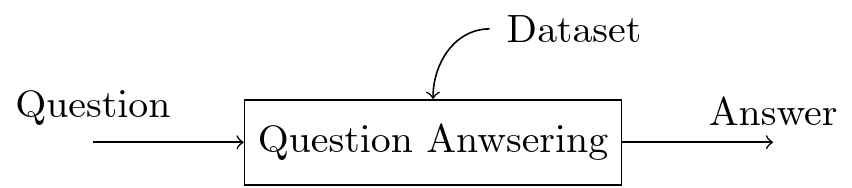
\includegraphics[width=\textwidth,height=2.1cm,keepaspectratio=true]{intro_qa}
    \caption{Suggested \gls{qa} diagram}
    \label{fig:intro_qa}
\end{figure}

\paragraph{Primaries}
\begin{itemize}[noitemsep]
    \item Select existing papers and projects treating the subject as a starting point.
    \item Identify relevant datasets.
    \item Develop one or more \gls{poc}.
    \item Test and evaluate solutions.
    \item Suggest improvements, possible continuation, and future outcomes.
\end{itemize}
\paragraph{Secondaries}
\begin{itemize}[noitemsep]
    \item Extend the \gls{qa} chatbot using "tailored" knowledge, e.g., \gls{model-ft} with press content.
\end{itemize}

\subsection{\gls{generative} \gls{qa} Chatbot}
The second objective is to extend the output from the \gls{qa} system, from the first objective, by enhancing the answers and generate human-like sentences from the enhanced answers. The initial vision for this objective is as illustrated in Figure~\ref{fig:intro_qa_gen}, a two parts system. The \textit{Enricher} enriches the answer from the \gls{qa} system, e.g. using a knowledge base\footnote{Wikidata.org, a Freebase-based  \autocite{paper:bollacker2008} knowledge base or Google's Knowledge Graphs \autocite{blog:intro_knowledge_graph}}. The \textit{Generator} aims at creating readable text from the enriched answer. Besides, we could also use user profiles\footnote{Fictive profiles in the context of the thesis} as input to those two parts.
\begin{figure}[ht!]
    \centering
    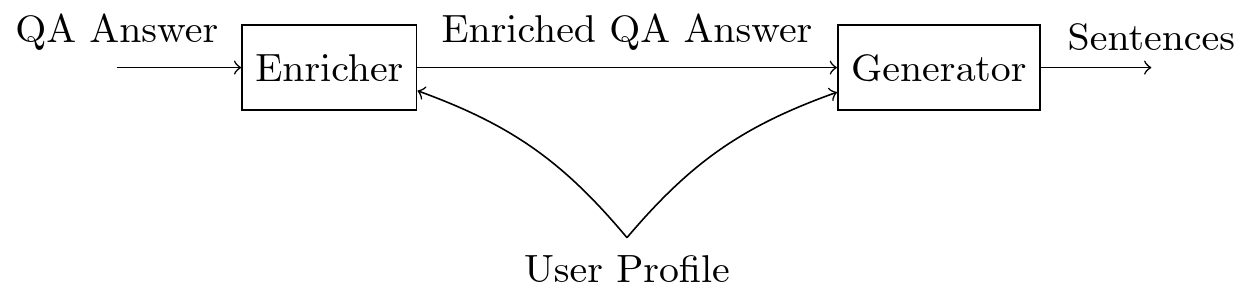
\includegraphics[width=\textwidth,keepaspectratio=true]{intro_qa_gen}
    \caption{Suggested \gls{generative} \gls{qa} diagram}
    \label{fig:intro_qa_gen}
\end{figure}


\paragraph{Primaries}
\begin{itemize}[noitemsep]
    \item Investigate a rule-based system for keyword enrichment.
    \item Generate sentences with keywords.
    \item Identify relevant datasets.
    \item Develop one or more \gls{poc}.
    \item Test and evaluate solutions.
    \item Suggest improvements, possible continuation, and future outcomes.
\end{itemize}
\paragraph{Secondaries}
\begin{itemize}[noitemsep]
    \item Use advanced strategies to enrich keywords.
    \item Use advanced text generation technics such as GTP-2\footnote{OpenAI's GTP-2 Algorithm \autocite{papers:gpt2}}.
    \item Use user profiles to customize the outputs.
\end{itemize}


\section{Initial Plan}
\label{plan:plan}
\subsection{Contraints}
\textbf{Timeframe:} 19 weeks\\
\textbf{Starting date:} 16.09.2019\\
\textbf{Ending date:} 07.02.2020

\subsection{Methodologies}
For consistency, the project is separated into two methodological parts. The first third, as the project targets information gathering and self-study, we use a standard sequential project management methodology. For the next two-thirds of the project, we will be using an agile methodology to perform incremental progress while exploring.

\subsubsection{Back to level Milestones}
First third of the study, from \textbf{16.09.19 to 25.10.19 (6 weeks)}.
\begin{enumerate}
    \setlength\itemsep{0em}
    \item[M1.] Initial \gls{mt} plan and project specification
    \item[M2.] Review the state of the art of the \gls{nlp} and \gls{nlu} technologies and refine the plan if needed.
\end{enumerate}


\subsubsection{Diving into the subject Milestones}
\textbf{From 28.10.19 to 07.02.20 (13 weeks)}, the following two-third of the work is composed of 6 sprints of two weeks each and one week to finalize the thesis.
\begin{itemize}
    \setlength\itemsep{0em}
    \item[M3.] Basic \gls{qa} Chatbot
    \item[M4.] Evaluation of basic \gls{qa} Chatbot
    \item[M5.] Basic generative \gls{qa} Chatbot
    \item[M6.] Evaluation of basic generative \gls{qa} Chatbot
\end{itemize}

\subsection{Gantt}
The Figure~\ref{fig:gantt-initial} represents the chart for the initial plan.

\newganttchartelement*{project-milestone}{
project-milestone/.style={
shape=isosceles triangle,
inner sep=0pt,
draw=cyan,
top color=white,
bottom color=cyan!50
},
project-milestone incomplete/.style={
/pgfgantt/project-milestone,
draw=yellow,
bottom color=yellow!50
},
project-milestone label font=\slshape,
project-milestone left shift=0pt,
project-milestone right shift=0pt
}

\newgantttimeslotformat{stardate}{
\def\decomposestardate##1.##2\relax{
\def\stardateyear{##1}\def\stardateday{##2}
}
\decomposestardate#1\relax
\pgfcalendardatetojulian{\stardateyear-01-01}{#2}
\advance#2 by-1\relax
\advance#2 by\stardateday\relax
}

\begin{figure}[h]%[htbp]
\centering
\begin{ganttchart}[vgrid, hgrid]{1}{19}
\gantttitle{Sep}{2} 
\gantttitle{Oct}{5}
\gantttitle{Nov}{4}
\gantttitle{Dec}{3}
\gantttitle{Jan}{4}
\gantttitle{Feb}{1}\\
\gantttitlelist{1,...,19}{1}\\

%part 1
\ganttgroup{Back to level}{1}{6} \\
\ganttmilestone{M1, M2}{3}
\ganttmilestone{}{6}\\

%part 2
\ganttgroup{Diving}{7}{18} \\
\ganttbar{Sprint 1}{7}{8} \\
\ganttbar{Sprint 2}{9}{10} \\
\ganttmilestone{M3}{10}\\
\ganttbar{Sprint 3}{11}{12} \\
\ganttmilestone{M4}{12}\\
\ganttbar{Sprint 4}{13}{14} \\
\ganttbar{Sprint 5}{15}{16} \\
\ganttmilestone{M5}{16}\\
\ganttbar{Sprint 6}{17}{18} \\
\ganttmilestone{M6}{18}\\

%\ganttlink{elem6}{elem7}
%\ganttlink{elem8}{elem9}

%part 3
\ganttgroup{Wrap up}{19}{19} \\


\end{ganttchart}

\caption{Initial Gantt Chart}
\label{fig:gantt-initial}
\end{figure}



\section{Tasks}
\label{chap:tasks}

\subsection{Initial Tasks}
\label{plan:initial-tasks}

\subsubsection{Primaries}
\begin{enumerate}
    \setlength\itemsep{0em}
    \item \gls{ai} in journalism state of the art
    \item \gls{nlp} and \gls{nlu} state of the art
    \item Find relevant datasets
    \item Find existing projects and papers responding to the questions
    \item Explore documents' topics extraction
    \item Explore the Wikidat and knowledge graphs
    \item Explore question-answering technologies and technics
    \item Evaluate by comparing to similar systems
\end{enumerate}
\paragraph{Milestones}
\begin{enumerate}
    \setlength\itemsep{0em}
    \item Initial \gls{mt} plan and project specification
    \item Overview topics extraction technics
    \item Overview Wikidata and knowledge graphs technics
    \item Overview text transformative and generative technics
    \item Mindmap of the current \gls{nlp} and \gls{nlu} technologies
    \item Pytorch hands-on
\end{enumerate}

\subsubsection{Secondaries}
\begin{itemize}
    \setlength\itemsep{0em}
    \item Explore \gls{ai} implications in journalism
    \item Explore \gls{ai} personalization implications
    \item Explore text generative technologies
    \item Explore profile-based customization
    \item Explore text transformative technologies
    \item Explore the attention mechanism
    \item Explore text summarization
    \item Explore text flavoring to write as a specific author
    \item Explore news extraction from social media
    \item Explore news baseline extraction
    \item Explore news drafts and briefs generation
    \item Explore text adapted suggestions for journalists
    \item Explore knowledge graphs as content enrichment
    \item Explore multiple sources cross-checking to reduce fake news
    \item Explore tracker for the original source
    \item Explore autonomous knowledge gathering
    \item Explore machine-generated factual discussions
    \item Explore machine self-training
    \item Explore chain reasoning
    \item Explore artificial common sense
    \item Explore artificial intuition
    \item Explore on the fly translations
    \item Make overall improvements
\end{itemize}
\paragraph{Milestones}
\begin{itemize}
    \setlength\itemsep{0em}
    \item Basic topic extraction from documents
    \item Basic conversational agent
    \item Basic journalistic agent
\end{itemize}
